\documentclass[journal]{IEEEtran}
\usepackage[utf8]{inputenc} % Codificación de entrada UTF-8
\usepackage{cite} % Para citaciones
\usepackage{placeins} % Para \FloatBarrier
\usepackage{graphicx} % Para incluir imágenes
\usepackage{float}
\usepackage{amsmath} % Para fórmulas matemáticas
\usepackage{url} % Para manejar URLs
\usepackage{listings}
\usepackage{xcolor}
\usepackage[ruled,vlined]{algorithm2e} % Para pseudocódigo
\usepackage{authblk}
\usepackage{hyperref}
\usepackage{breakurl}
\usepackage[spanish]{babel}

% Configuración de listings para bash
\lstset{
  language=bash,
  basicstyle=\ttfamily, 
  columns=fullflexible, 
  frame=single, 
  breaklines=true, 
  postbreak=\mbox{\textcolor{red}{$\hookrightarrow$}\space}, 
  backgroundcolor=\color{lightgray!20},  
  keywordstyle=\color{blue}, 
  commentstyle=\color{green}, 
  stringstyle=\color{red} 
}

\title{Especificación Formal y Validación para la Prevención de Colisiones en Tráfico Ferroviario}
\author[1]{Infanzón Acosta R. E.}
\author[1]{Aguilar Chirinos C. D.}
\author[1]{Quispe Huanca A. M.}
\affil{Universidad La Salle, Arequipa, Perú}



\author[2]{Molina Barriga M. - Mentor }

\begin{document} 

\maketitle

\begin{abstract}
Aquí el Abtract o resumen
\end{abstract}

\begin{IEEEkeywords}
Aquí las Keywords
\end{IEEEkeywords}

\section{Introducción}  
La seguridad en el transporte ferroviario es un aspecto crítico para garantizar el bienestar de las personas que utilizan este medio de transporte a diario. Según el \textit{Informe sobre la Seguridad y la Interoperabilidad Ferroviaria en la UE 2024}, el sistema ferroviario de la UE se considera uno de los más seguros del mundo. Sin embargo, a pesar de la disminución de accidentes significativos desde 2010, se ha registrado un aumento en 2021 y 2022, alineándose con los niveles pre-pandemia de COVID-19. Esta realidad se ve agravada por el estancamiento de las tasas de fatalidades de pasajeros desde 2017 \cite{eu2024}. Las repercusiones de estos incidentes se extienden más allá de los pasajeros y trabajadores, afectando profundamente a las comunidades y economías que dependen del ferrocarril \cite{carrington2019}.  

Ante esta situación, es fundamental explorar nuevas estrategias para prevenir colisiones y reforzar un sistema más seguro. La implementación de tecnologías avanzadas en el ámbito de la seguridad ferroviaria se ha convertido en una prioridad. Investigaciones recientes indican que la evolución de las tecnologías de seguridad está proporcionando respuestas más efectivas ante situaciones peligrosas \cite{ong2021risk}. En este contexto, se busca desarrollar un mecanismo que minimice el riesgo de colisiones y reduzca los errores humanos y las fallas en la comunicación dentro del sistema ferroviario. La automatización de tareas críticas, como la detección de trenes en las vías y el control de su velocidad, es esencial para una respuesta adecuada ante situaciones potencialmente peligrosas \cite{automation2020}.  

Además, será necesario diseñar un modelo formal que estructure y analice la información relacionada con la seguridad ferroviaria, asegurando así la precisión y la integridad de los datos utilizados en la prevención de colisiones. Este enfoque permitirá mejorar la identificación de situaciones de riesgo y sentar las bases para futuras herramientas de mejora en la seguridad ferroviaria.  

\subsection{Alcance esperado}
El alcance de este proyecto se centra en la aplicación de métodos formales para estructurar y analizar el sistema de prevención de colisiones ferroviarias. A través del uso de VDM++ y model-checking, se busca desarrollar un modelo formal que permita verificar la consistencia y validez de las interacciones entre los componentes del sistema, como los trenes y sensores. Este enfoque garantizará la integridad de las decisiones automatizadas, como los cambios de señales o ajustes de velocidad, y asegurará que el sistema funcione correctamente en todas las condiciones posibles. Mediante un análisis riguroso y sistemático, se contribuirá a mejorar la seguridad del tráfico ferroviario, proporcionando una base sólida para el desarrollo de herramientas futuras que optimicen la prevención de accidentes en el ámbito ferroviario.

\section{Resumen Ejecutivo}

\subsection{Antecedentes}
\subsubsection{Un Sistema de Seguridad y Prevención de Colisiones en Tiempo Real para Trenes}
\subsubsection*{Resumen}  
El artículo presenta un sistema integral de seguridad que combina diversas tecnologías avanzadas para la prevención de colisiones en el transporte ferroviario. Reconoce que, a pesar de las mejoras en la infraestructura y las técnicas de gestión, los peligros persisten, lo que justifica la implementación de un enfoque más proactivo. El sistema propuesto utiliza datos en tiempo real para detectar y responder a situaciones de riesgo, con el fin de prevenir accidentes antes de que ocurran. Además, se subraya la importancia de la comunicación entre trenes, estaciones y otros elementos del sistema para asegurar una operación sincronizada y segura.
\subsubsection*{Puntos de interés para la investigación}  
\begin{itemize}
    \item \textbf{Detección y Respuesta en Tiempo Real:}  
    Según Wu (2017), el sistema se basa en tecnologías de detección que permiten identificar situaciones peligrosas en tiempo real, activando respuestas automáticas como la reducción de velocidad o la detención total antes de que se produzca una colisión \cite{railwaycouncil2017realsafetysystem}.    
    \item \textbf{Integración de Tecnologías Avanzadas:}  
    Wu (2017) destaca que se integran tecnologías como el monitoreo por GPS, sensores de proximidad y sistemas de comunicación entre trenes, lo que mejora la conciencia situacional y la capacidad de respuesta ante emergencias \cite{railwaycouncil2017realsafetysystem}.    
    \item \textbf{Comunicaciones Eficientes:}  
    Según Wu (2017), la comunicación efectiva entre los trenes y las estaciones es clave para coordinar acciones y minimizar riesgos. El autor resalta la necesidad de protocolos de comunicación robustos para asegurar que la información crítica se transmita sin demora \cite{railwaycouncil2017realsafetysystem}.   
    \item \textbf{Beneficios Socioeconómicos:}  
    Wu (2017) señala que, al reducir la frecuencia y severidad de los accidentes, el sistema no solo mejora la seguridad de los pasajeros y el personal, sino que también tiene beneficios económicos para las comunidades dependientes del transporte ferroviario, al mitigar pérdidas asociadas a accidentes y paradas operativas \cite{railwaycouncil2017realsafetysystem}.    
    \item \textbf{Evaluación Continua y Mejora del Sistema:}  
    Según Wu (2017), el sistema incluye mecanismos para la evaluación continua y la mejora de los procedimientos de seguridad, asegurando que se mantenga actualizado frente a nuevas amenazas y desarrollos tecnológicos en el ámbito ferroviario \cite{railwaycouncil2017realsafetysystem}.
\end{itemize}

\subsubsection{SafeCap: Un Sistema de Seguridad para la Prevención de Colisiones en Tráfico Ferroviario}
\subsubsection*{Resumen}  
El documento presenta el sistema SafeCap, diseñado específicamente para abordar la seguridad en las operaciones ferroviarias y evitar colisiones entre trenes. A pesar de las mejoras en la infraestructura ferroviaria y las tecnologías actuales, los accidentes siguen siendo una preocupación significativa. SafeCap utiliza sensores y tecnología de comunicación para proporcionar un monitoreo continuo del estado de los trenes y su entorno. El sistema puede detectar situaciones potencialmente peligrosas y activar alertas o intervenciones automáticas para prevenir colisiones.
\subsubsection*{Puntos de interés para la investigación}  
\begin{itemize}
    \item \textbf{Detección Proactiva de Riesgos:}  
    Hann y Couch (2014) afirman que SafeCap implementa tecnologías de detección avanzada que permiten identificar riesgos en tiempo real, lo que facilita una respuesta rápida ante situaciones peligrosas y garantiza la seguridad de los viajeros y el personal \cite{ada2014safecap}.   
    \item \textbf{Integración de Sensores y Sistemas de Comunicación:}  
    Los autores destacan que el sistema hace uso de diversos sensores que recopilan datos críticos y los transmiten a través de redes seguras, asegurando que la información relevante esté disponible de manera inmediata, lo que mejora la toma de decisiones en situaciones de emergencia \cite{ada2014safecap}.    
    \item \textbf{Intervenciones Automáticas:}  
    Hann y Couch (2014) subrayan que una característica clave de SafeCap es la capacidad de llevar a cabo intervenciones automáticas, como frenar o desviar trenes, a fin de evitar accidentes. Esto reduce la dependencia de la intervención humana y el margen de error asociado \cite{ada2014safecap}.   
    \item \textbf{Mejora Continua del Sistema:}  
    Según los autores, SafeCap incluye un enfoque de mejora continua que permite al sistema aprender de incidentes previos y ajustarse para optimizar su rendimiento, asegurando que se mantenga actualizado frente a nuevas amenazas \cite{ada2014safecap}.  
    \item \textbf{Impacto Social y Económico:}  
    Hann y Couch (2014) mencionan que la implementación de SafeCap no solo incrementa la seguridad en el transporte ferroviario, sino que también tiene un impacto positivo en las comunidades, al reducir los costos económicos relacionados con accidentes y mejorar la confianza del público en el sistema ferroviario \cite{ada2014safecap}.
\end{itemize}
\subsubsection{Intel: Sistemas de Prevención de Colisiones en Trenes}
\subsubsection*{Resumen}  
El informe detalla la importancia de los sistemas de prevención de colisiones en el contexto del transporte ferroviario. A pesar de que el medio ferroviario es considerado uno de los más seguros, los accidentes continúan representando una amenaza significativa. Los sistemas de prevención de colisiones utilizan tecnología de monitoreo y comunicación para identificar y mitigar riesgos en tiempo real, permitiendo la intervención automática ante situaciones de peligro. Esto no solo ayuda a evitar accidentes, sino que también optimiza las operaciones del servicio ferroviario.
\subsubsection*{Puntos de interés para la investigación}  
\begin{itemize}
    \item \textbf{Monitoreo en Tiempo Real:}  
    Intel (2022) explica que los sistemas de prevención de colisiones se basan en tecnologías de monitoreo en tiempo real, lo que permite la evaluación constante de las condiciones operativas y la detección de situaciones de riesgo, asegurando respuestas rápidas ante emergencias \cite{intel2022collision}.   
    \item \textbf{Interconexión de Sistemas:}  
    El autor enfatiza la importancia de la interconexión entre diferentes componentes del sistema ferroviario, como señales, trenes y centros de control, para una comunicación efectiva. Esta integración es esencial para coordinar acciones preventivas y garantizar una respuesta ágil ante cualquier riesgo \cite{intel2022collision}.    
    \item \textbf{Intervenciones Automáticas:}  
    Según Intel (2022), los sistemas son capaces de implementar intervenciones automáticas, como el frenado o cambios de ruta, cuando se detectan condiciones peligrosas. Esto reduce la dependencia del operador humano y minimiza el margen de error \cite{intel2022collision}.  
    \item \textbf{Compatibilidad con Nuevas Tecnologías:}  
    Intel (2022) también destaca cómo los sistemas de prevención de colisiones pueden integrarse con tecnologías emergentes, como inteligencia artificial y análisis de datos, para mejorar su eficacia y adaptabilidad ante nuevos desafíos \cite{intel2022collision}.
    \item \textbf{Beneficios Económicos y Sociales:}  
    El autor señala que la reducción de accidentes no solo tiene un impacto positivo en la seguridad de los usuarios, sino que también contribuye a la eficiencia económica del transporte ferroviario, disminuyendo costos asociados a paradas no planificadas y daños. Esto fomenta la confianza pública en los viajes en tren, beneficiando a las comunidades y economías locales \cite{intel2022collision}.
\end{itemize}

\section{Requerimientos funcionales}

\subsubsection{Detección de ocupación de vías} 
El sistema debe ser capaz de detectar de manera precisa si una vía está ocupada por un tren u objeto, y debe activar automáticamente los semáforos correspondientes para evitar que un tren entre en una vía ocupada.

\subsubsection{Cálculo de distancia entre trenes} 
El sistema debe medir continuamente la distancia entre trenes en circulación para garantizar que se mantenga una distancia de seguridad adecuada, y debe alertar o activar mecanismos de frenado si la distancia se reduce a niveles peligrosos.

\subsubsection{Ajuste automático de velocidad} 
El sistema debe ser capaz de ajustar la velocidad de los trenes en función de las condiciones de la vía, como la proximidad a otros trenes, la ocupación de las vías y otros factores relevantes, para garantizar que los trenes puedan frenar de manera segura en situaciones críticas.

\subsubsection{Control de la integridad de la vía} 
El sistema debe supervisar continuamente el estado de la infraestructura ferroviaria, incluyendo las vías, para detectar fallos estructurales o desviaciones que puedan comprometer la seguridad, y activar medidas preventivas en caso de identificar un problema.

\subsubsection{Verificación en tiempo real} 
El sistema debe ser capaz de verificar en tiempo real las decisiones tomadas por los sensores y los semáforos, las acciones que se basen en datos correctos y precisos, y proporcionar informes de error si se detectan inconsistencias o fallos en el proceso.

\section{Objetivos de la investigación}  
\subsection{Objetivo general}  
Diseñar un modelo formal con VDM++ que estructure y analice la información relacionada con la seguridad ferroviaria, incluyendo datos de ocupación de vías, distancias entre trenes y estados de sensores, para garantizar la precisión, coherencia e integridad de los datos utilizados en la prevención de colisiones. Esto facilitará un análisis preciso y sistemático, mejorando la identificación de situaciones de riesgo y estableciendo las bases para futuras herramientas de mejora en la seguridad ferroviaria.  

\subsection{Objetivos Específicos}  

\begin{itemize}  
    \item Crear un modelo formal en VDM++ que organice y represente de manera precisa los datos de ocupación de vías y distancias entre trenes, asegurando la coherencia de la información en el análisis de la seguridad ferroviaria.  

    \item Diseñar un procedimiento formal que evalúe la coherencia temporal de los eventos en el sistema de prevención de colisiones, verificando que las decisiones, como el ajuste de velocidad, se realicen en un orden lógico y consistente, y detectando posibles discrepancias en la comunicación del sistema.  

    \item Desarrollar un método de validación que garantice que la información sobre la ocupación de vías y el estado del sistema no haya sido alterada ni corrompida, asegurando que los datos utilizados en el análisis de seguridad sean válidos y confiables en todas las etapas del procedimiento.  

    \item Evaluar el impacto del modelo desarrollado en la precisión y eficiencia de la prevención de colisiones ferroviarias, estableciendo las bases para el desarrollo de futuras herramientas especializadas que optimicen el procesamiento y análisis de datos de seguridad ferroviaria.  
\end{itemize}  

\section{Metodología}  

La presente investigación se enmarca en el contexto de la creciente necesidad de mejorar la seguridad ferroviaria, con énfasis en la prevención de colisiones. La elección de datos sobre ocupación de vías y distancias entre trenes como fuente primaria responde a su relevancia en la identificación de situaciones de riesgo y en la mejora de la gestión del tráfico ferroviario.  

Se emplean técnicas avanzadas de formalización de software, específicamente el uso de VDM++ y model checking, que garantizan la consistencia y precisión en el análisis. Estas herramientas permiten modelar de manera adecuada las relaciones temporales y los eventos registrados, asegurando que las evidencias sean confiables y verificables en el ámbito de la seguridad ferroviaria, así como establecer un precedente para una construcción adecuada de estrategias de prevención.  

El diseño cualitativo y el enfoque formal elegido se justifica por su capacidad de estructurar información compleja, ordinal y fragmentada, maximizando su validez para establecer conclusiones en los resultados obtenidos y contribuir al desarrollo de procedimientos estandarizados en el análisis de datos de seguridad ferroviaria.  

\subsubsection*{Método investigativo}  
El método empleado en esta investigación se centra en la interpretación y análisis de datos de ocupación de vías y distancias entre trenes. Estos datos se abstraen para facilitar su comprensión por sistemas computacionales y establecer relaciones entre ellos, permitiendo la formulación de un caso basado en las características específicas de cada tipo de registro, ahora definidos como clases. El objetivo principal es identificar patrones significativos y evaluar situaciones de riesgo asociadas a la operación ferroviaria.  

Los datos que se tendrán en cuenta para ser analizados en el modelo provienen de fuentes pertinentes, como registros de telecomunicaciones ferroviarias y documentos oficiales de investigaciones previas. En el modelo, estos datos son procesados mediante técnicas formales, utilizando modelos en VDM++ y herramientas de model checking, que están ligadas a estados dentro de las operaciones de cada una de las clases (registros), lo que permite evaluar la coherencia temporal y la validez de los eventos registrados.  

Finalmente, se concluye que este método de enfoque cualitativo sobresale por su capacidad de abordar información incompleta y garantizar precisión en la reconstrucción de eventos, contribuyendo significativamente al desarrollo de procedimientos de seguridad más eficientes y adaptables, lo que representa una adecuada base para proceder con esta investigación.  

\subsection*{Procedimiento de Investigación}  
En el repositorio de GitHub se tiene el código completo de la investigación, que está basado en el modelado formal de datos relacionados con la seguridad ferroviaria utilizando el lenguaje VDM++.\cite{rodrigostranger2023trafico_de_trenes}\\
A continuación, se presenta una imagen básica del modelado de clases que muestra las principales clases involucradas en la estructura del modelo. Esta imagen ilustra cómo se organizan las clases de datos en el modelo propuesto.  

\begin{figure}[htbp]
    \centering
    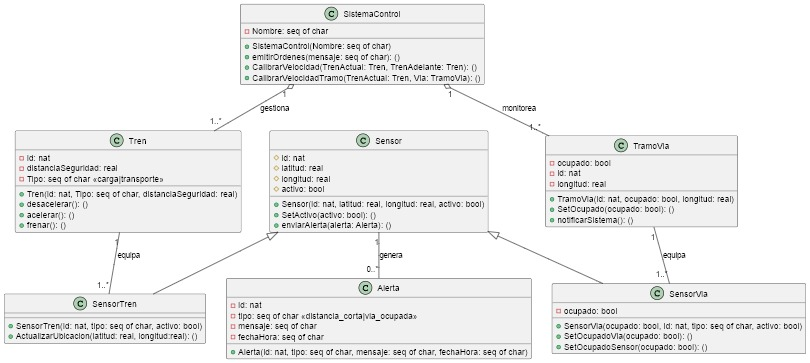
\includegraphics[width=0.4\textwidth]{img/diagrama-clases.jpg}
    \caption{Modelo de datos generado por VDM}
    \label{fig:VDM_model}
\end{figure} 

\bibliographystyle{IEEEtran}
\sloppy
\bibliography{citas}

\end{document}
